% ══════════════════════════════════════════════════════════════════════════════
%  CAPITOLO — FIDELIZZAZIONE DEI DONATORI GIOVANI
%  Etichette: ch:retention, sec:ret_def, sec:ret_ident, sec:ret_dist,
%             sec:ret_survival, sec:ret_gender, sec:ret_comparison,
%             sec:ret_summary
% ══════════════════════════════════════════════════════════════════════════════

\chapter{Fidelizzazione dei Donatori Giovani}
\label{ch:retention}

La tenuta del sistema trasfusionale dipende non solo dal reclutare donatori ma
soprattutto dal \emph{trattenerli}. Il \cref{ch:eda} ha mostrato che gli
ingressi calano e che l'intensità individuale non compensa: resta da capire
quanto rapidamente si perde chi entra. La fascia d'ingresso \textbf{18--25
anni} ha un interesse particolare, perché chi inizia da giovane ha davanti il
massimo orizzonte di attività e, se fidelizzato, contribuisce per decenni; ed è
anche la fascia in cui l'abbandono dopo la prima donazione è tipicamente più
alto, per la mobilità geografica legata a studio e lavoro e per la minore
radicazione nelle reti associative.

Il capitolo misura quanti donatori giovani tornano, per quanti anni restano
attivi, se ci sono differenze fra maschi e femmine e come si collocano rispetto
a chi inizia in età più matura. Prima di tutto questo, però, va risolto un
problema di definizione che condiziona ogni numero del capitolo.

% ───────────────────────────────────────────────────────────────────────
\section{Chi è una coorte di ingresso}
\label{sec:ret_def}

Si definisce \textbf{donatore giovane} chi effettua la prima donazione fra i 18
e i 25 anni compiuti. La soglia inferiore è il limite legale in Italia; quella
superiore include l'intera finestra di transizione scuola--lavoro, ed è
coerente con la letteratura internazionale sulla donazione
giovanile~\cite{Maghsudlu2017}.

Il punto delicato è cosa si intende per \emph{prima} donazione. La finestra
osservata comincia nel 2009, ma il sistema trasfusionale no: come anticipato
nella \cref{sec:temporal}, dove due terzi dei ``nuovi'' del 2009 risultano già
attivi, il $30{,}4\%$ dei donatori presenti nel dataset aveva già cominciato a
donare prima del 2009. Per costoro la prima donazione
\emph{osservata} non è la prima donazione, e il primo anno in cui compaiono non
è il loro anno di ingresso.

L'errore non è innocuo, perché non è distribuito a caso: chi viene intercettato
a metà carriera è, per costruzione, un donatore che è già sopravvissuto alla
selezione per abbandono precoce, e quindi sopravvive più a lungo di una recluta
vera. Includerlo in una coorte di ingresso gonfia sistematicamente la curva di
sopravvivenza di quella coorte. Il problema è massimo proprio nella coorte
2009.

\begin{table}[ht]
\centering
\caption{Quota di ciascuna coorte apparente costituita in realtà da donatori
già attivi prima del loro primo anno osservato.}
\label{tab:coorti_composizione}
\begin{tabular}{@{}rrr@{\qquad}rrr@{}}
\toprule
\textbf{Coorte} & \textbf{Donatori} & \textbf{Già attivi} &
\textbf{Coorte} & \textbf{Donatori} & \textbf{Già attivi} \\
\midrule
\textbf{2009} & 1\,970 & \textbf{50{,}5\%} & 2016 & 943 & 12{,}7\% \\
2010 & \phantom{0}908 & 28{,}9\% & 2017 & 743 & 13{,}7\% \\
2011 & 1\,000 & 14{,}1\% & 2018 & 996 & 10{,}4\% \\
2012 & \phantom{0}972 & \phantom{0}8{,}2\% & 2019 & 764 & 10{,}7\% \\
2013 & \phantom{0}791 & 10{,}4\% & 2020 & 520 & 18{,}7\% \\
2014 & \phantom{0}810 & 13{,}8\% & 2021 & 566 & 14{,}5\% \\
2015 & \phantom{0}980 & 12{,}4\% & 2022 & 694 & 10{,}5\% \\
     &                &          & 2023 & 755 & \phantom{0}9{,}5\% \\
\bottomrule
\end{tabular}
\end{table}

La \cref{tab:coorti_composizione} rende la scala del problema: la coorte 2009 è
per \textbf{metà} composta da donatori già attivi, quella 2010 per oltre un
quarto, e dal 2011 in poi la quota oscilla fra l'8 e il 19 per cento, in
genere fra il 10 e il 14.
Ed è proprio la coorte 2009 quella che verrebbe naturale usare come esempio
principale delle curve di sopravvivenza, perché è la più numerosa e la più
lunga: è la coorte su cui l'errore pesa di più.

\paragraph{La correzione adottata.}
Nel seguito la coorte di ingresso comprende \textbf{soltanto i donatori la cui
attività comincia davvero dentro la finestra osservata}, cioè quelli per cui la
data di inizio attività è nota e cade nell'anno del primo evento registrato.
Escono dal calcolo due gruppi: i troncati a sinistra, che non appartengono in
senso proprio ad alcuna coorte osservabile, e --- necessariamente --- quelli
per cui la data di inizio \emph{manca}, di cui non si può dire se siano
reclute o veterani. Il secondo gruppo è la ragione per cui i conteggi di questo
capitolo non si ottengono sottraendo le quote della
\cref{tab:coorti_composizione} dai totali: la coorte 2009, ad esempio, conta
1\,970 donatori apparenti, di cui 994 già attivi prima e 185 senza data, e ne
restano 791 genuini. È anche il motivo per cui la serie di ingressi del
\cref{ch:eda}, che adotta il criterio più permissivo, è più alta di questa.

Va scartata invece una correzione che verrebbe naturale --- usare la data di
inizio attività come anno di ingresso e ricalcolare la retention da lì. Per chi
ha cominciato nel 2004 ed è osservato dal 2009 quel calcolo conterebbe cinque
anni di attività che nel dataset non ci sono, e produrrebbe una retention
\emph{più alta} di quella osservabile per una ragione puramente contabile. Le
due definizioni effettivamente adottate --- prima donazione osservata e solo
ingressi genuini --- sono calcolate entrambe per ogni misura del capitolo; 
nel testo si usa la seconda.

% ───────────────────────────────────────────────────────────────────────
\section{Consistenza del gruppo}
\label{sec:ret_ident}

Restringendo alle coorti 2009--2023 e osservando fino al 2025 --- così che
ogni coorte abbia almeno due anni di osservazione successiva --- il dataset
contiene \textbf{21\,085 ingressi genuini}. Di questi, \textbf{10\,552} sono
avvenuti fra i 18 e i 25 anni: \textbf{il 50{,}0\%} degli ingressi. I donatori
giovani così definiti generano \textbf{44\,237 donazioni} nel periodo osservato.

Il dato merita una sottolineatura, perché ribalta un'impressione: guardando
tutti i donatori presenti nel dataset i giovani sono un terzo, ma guardando
\emph{chi entra} sono la metà. Combinato con il risultato della
\cref{sec:denominatore} --- a parità di popolazione i 20--24enni sono la fascia
che dona di più --- il quadro è che il reclutamento giovanile funziona. È dopo
che si perde.

% ───────────────────────────────────────────────────────────────────────
\section{Distribuzione della retention}
\label{sec:ret_dist}

Per ogni donatore giovane si calcola la \textbf{retention}
$r = \text{ultimo anno} - \text{primo anno}$, cioè la distanza in anni fra
l'anno della prima e quello dell'ultima donazione osservata
(\cref{tab:ret_dist}). La misura è per anni solari: $r = 0$ indica chi dona in
un solo anno e non torna negli anni successivi, anche se in quell'anno ha
donato più di una volta.

\begin{table}[ht]
\centering
\caption{Distribuzione della retention per i 10\,552 donatori giovani entrati
fra il 2009 e il 2023, osservati fino al 2025.}
\label{tab:ret_dist}
\begin{tabular}{@{}rrrr@{}}
\toprule
\textbf{Anni di retention} & \textbf{Donatori} & \textbf{\%} & \textbf{\% cumulata} \\
\midrule
0  (un solo anno)      & 4\,281 & 40{,}6 & 40{,}6 \\
1                      & 1\,238 & 11{,}7 & 52{,}3 \\
2                      & \phantom{0}906 & \phantom{0}8{,}6 & 60{,}9 \\
3                      & \phantom{0}700 & \phantom{0}6{,}6 & 67{,}5 \\
4                      & \phantom{0}590 & \phantom{0}5{,}6 & 73{,}1 \\
5--9                   & 1\,819 & 17{,}2 & 90{,}4 \\
10+                    & 1\,018 & \phantom{0}9{,}6 & 100{,}0 \\
\midrule
\textbf{Totale}        & \textbf{10\,552} & \textbf{100{,}0} & \\
\bottomrule
\end{tabular}
\end{table}

Il risultato principale è la quota di donatori \textbf{``mordi e fuggi''}
($r = 0$): \textbf{il 40{,}6\%}. Due donatori giovani su cinque non tornano
negli anni successivi al primo (il $37{,}2\%$ dona una volta sola in assoluto).
Aggiungendo chi torna per un solo anno si arriva al \textbf{52{,}3\%}, che non
dona più dopo il secondo anno. All'altro estremo, il $26{,}9\%$ resta attivo
cinque anni o più e il $9{,}6\%$ almeno dieci --- un nucleo consolidato che
costituisce la componente strutturale del sistema.

Il numero mediano di donazioni per donatore giovane è \textbf{2} (media
$4{,}19$, deviazione standard $5{,}72$), con una coda che arriva a 122 donazioni
per il più assiduo: la stessa asimmetria della \cref{sec:intensity}.

% ───────────────────────────────────────────────────────────────────────
\section{Curve di sopravvivenza per coorte}
\label{sec:ret_survival}

Data la coorte entrata nell'anno $c$, si calcola la proporzione ancora attiva
nell'anno $c+k$. L'analisi è limitata alle coorti 2009--2018, per garantire un
orizzonte osservativo di almeno cinque anni.

La \cref{fig:ret_young} mostra a destra il confronto che vale la pena fare: la
coorte 2009 sotto le due definizioni, contro la banda di tutte le altre coorti.
Contando come coorte tutti i donatori al primo evento osservato, quella coorte
appare \emph{sopra} ogni altra a tutti gli orizzonti; sui soli ingressi
genuini rientra esattamente nella banda. Non era una
coorte più fedele: era mezza coorte di veterani.

\begin{table}[ht]
\centering
\caption{Sopravvivenza della coorte 2009 di donatori giovani, sotto le due
definizioni.}
\label{tab:ret_2009}
\begin{tabular}{@{}lrrrr@{}}
\toprule
& \textbf{1° anno} & \textbf{3° anno} & \textbf{5° anno} & \textbf{10° anno} \\
\midrule
Primo evento osservato ($n=1\,970$) & $54{,}0\%$ & $38{,}7\%$ & $25{,}9\%$ & $17{,}3\%$ \\
Soli ingressi genuini ($n=791$)     & $\mathbf{46{,}1\%}$ & $\mathbf{28{,}8\%}$ & $\mathbf{16{,}8\%}$ & $\mathbf{11{,}8\%}$ \\
\bottomrule
\end{tabular}
\end{table}

Lo scarto è sostanziale: al quinto anno la sopravvivenza misurata sui soli
ingressi genuini è \textbf{un terzo più bassa} (\cref{tab:ret_2009}).

\begin{figure}[H]
    \centering
    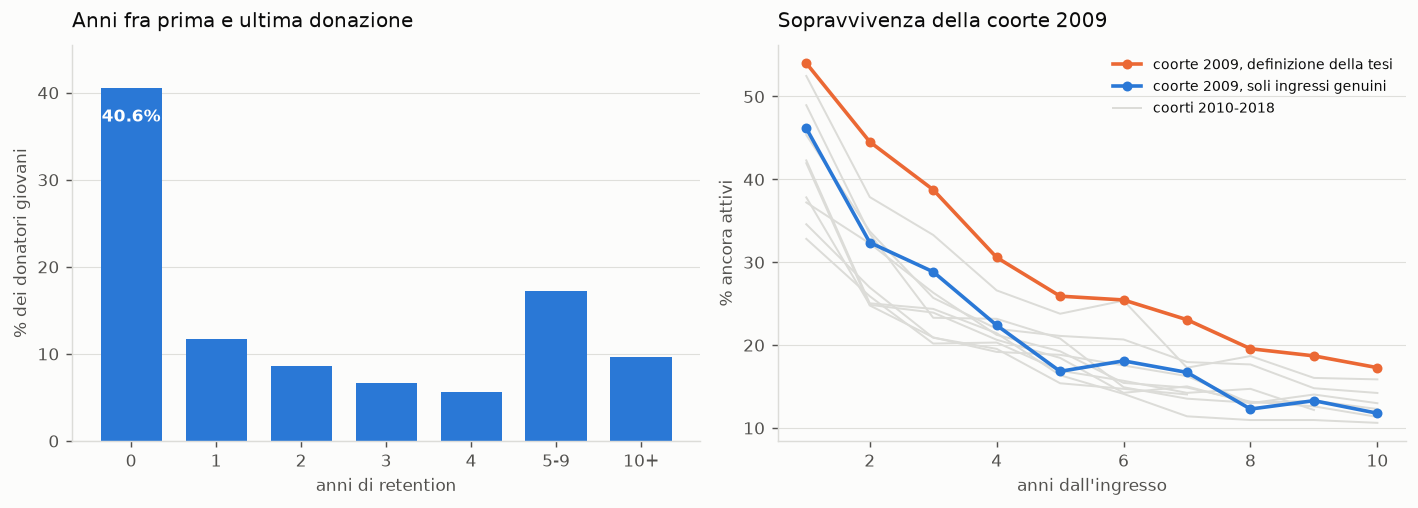
\includegraphics[width=0.95\linewidth]{img/fig_young_retention.png}
    \caption{Sinistra: distribuzione degli anni di retention. Destra:
    sopravvivenza della coorte 2009 sotto le due definizioni, sullo sfondo
    delle coorti 2010--2018.}
    \label{fig:ret_young}
\end{figure}

Quello che invece \textbf{non} cambia è la forma della curva, ed è la
conclusione sostantiva del capitolo: l'abbandono è \emph{frontalmente
caricato}. La perdita più consistente avviene fra il primo e il secondo anno,
e la perdita annua si riduce man mano che il donatore accumula anni. Il
pattern è coerente con una logica a \emph{soglia}: superati i primi anni, il
comportamento tende a stabilizzarsi come abitudine. Dal
punto di vista delle politiche di reclutamento ne segue che l'investimento più
efficace è quello sul \emph{secondo contatto}, cioè sul richiamo dei giovani
già donatori che non si sono ancora ripresentati.

La \cref{fig:ret_byage} mostra che la forma è la stessa per tutte le fasce
d'ingresso: la curva dei 18--25 sta sotto le altre, ma tutte decrescono con lo
stesso profilo frontalmente caricato, con la perdita maggiore fra il primo e il
secondo anno. É la dinamica
dell'ingresso; nei giovani cambia il livello: fa eccezione la
fascia 50+, che parte alta e scende più rapidamente delle altre fino a
incrociarle intorno al sesto anno --- coerentemente con il fatto che chi entra
oltre i cinquant'anni ha comunque davanti un orizzonte di idoneità più breve.

\begin{figure}[H]
    \centering
    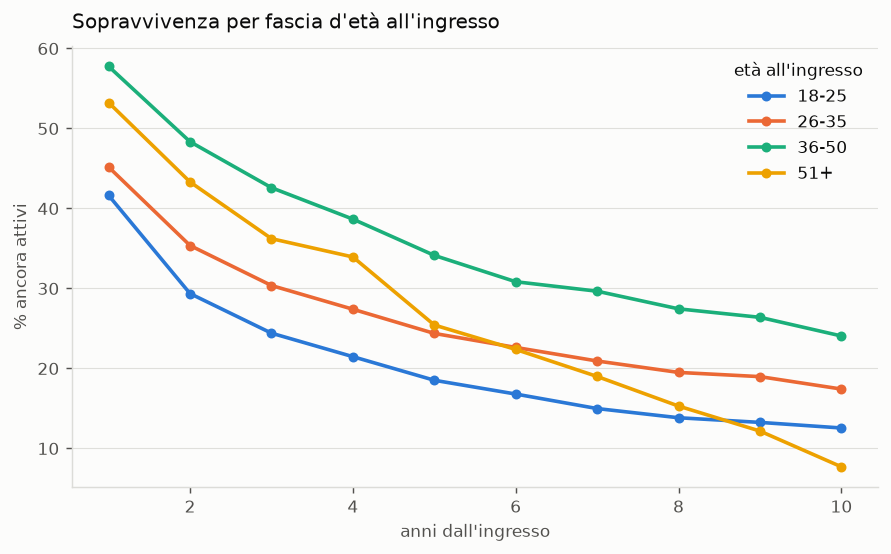
\includegraphics[width=0.90\linewidth]{img/fig_retention_by_age.png}
    \caption{Curve di sopravvivenza per fascia d'età all'ingresso, sui soli
    ingressi genuini.}
    \label{fig:ret_byage}
\end{figure}

% ───────────────────────────────────────────────────────────────────────
\section{Differenze di genere}
\label{sec:ret_gender}

Il gruppo dei donatori giovani è composto da \textbf{5\,786 maschi ($54{,}8\%$)}
e \textbf{4\,766 femmine ($45{,}2\%$)}, un rapporto molto meno squilibrato di
quello della popolazione donante complessiva (M/F $= 1{,}61$,
\cref{sec:demo}): il reclutamento giovanile coinvolge le donne in misura
relativamente maggiore rispetto alle fasce mature.

Le differenze di retention sono modeste ma coerenti (\cref{tab:ret_gender}): i
maschi hanno una retention media leggermente superiore ($3{,}24$ contro
$2{,}84$ anni) e una quota di \emph{one-timer} inferiore ($39{,}6\%$ contro
$41{,}7\%$). In entrambi i generi la mediana è 1 anno e il
75\textsuperscript{o} percentile è 5.

\begin{table}[ht]
\centering
\caption{Retention per genere, donatori giovani (soli ingressi genuini).}
\label{tab:ret_gender}
\begin{tabular}{@{}lrrrrrr@{}}
\toprule
\textbf{Genere} & \textbf{N} & \textbf{Media} & \textbf{DS} &
\textbf{Mediana} & \textbf{P75} & \textbf{One-timer} \\
\midrule
Maschi  (M) & 5\,786 & $3{,}24$ & $4{,}15$ & 1 & 5 & $39{,}6\%$ \\
Femmine (F) & 4\,766 & $2{,}84$ & $3{,}70$ & 1 & 5 & $41{,}7\%$ \\
\midrule
\textbf{Totale} & \textbf{10\,552} & $3{,}06$ & $3{,}96$ & 1 & 5 & $\mathbf{40{,}6\%}$ \\
\bottomrule
\end{tabular}
\end{table}

Il divario di $2{,}1$ punti percentuali è troppo contenuto per giustificare
strategie di retention differenziate per genere. Nelle analisi del
\cref{ch:glm} il genere entra quindi come covariata di controllo, non come
variabile di stratificazione --- il che è anche coerente con il fatto, discusso
nella \cref{sec:glm_effects}, che l'effetto del genere sulla \emph{frequenza} è
in larga parte un vincolo normativo e non una differenza di propensione.

% ───────────────────────────────────────────────────────────────────────
\section{Confronto con i donatori adulti}
\label{sec:ret_comparison}

I \textbf{10\,533 donatori adulti} (ingresso a 26 anni o più) permettono di
contestualizzare il risultato. Qui la correzione della coorte cambia
sensibilmente la conclusione (\cref{tab:ret_fasce}).

\begin{table}[ht]
\centering
\caption{Quota di \emph{one-timer} per fascia d'età all'ingresso, contando
come ingresso il primo evento osservato e contando invece i soli ingressi
genuini.}
\label{tab:ret_fasce}
\begin{tabular}{@{}lrr@{}}
\toprule
\textbf{Fascia d'ingresso} & \textbf{Primo evento oss.} & \textbf{Ingressi genuini} \\
\midrule
18--25 & $39{,}1\%$ & $40{,}6\%$ \\
26--35 & $31{,}1\%$ & $38{,}1\%$ \\
36--50 & $22{,}1\%$ & $28{,}2\%$ \\
51+    & $27{,}7\%$ & $33{,}1\%$ \\
\midrule
\emph{aggregato 26+} & $26{,}2\%$ & $33{,}3\%$ \\
\midrule
\textbf{rapporto giovani\,/\,adulti} & $\mathbf{1{,}49}$ & $\mathbf{1{,}22}$ \\
\bottomrule
\end{tabular}
\end{table}

Il divario esiste ancora --- i giovani abbandonano più spesso degli adulti ---
ma è \textbf{molto più piccolo di quanto la misura ingenua suggerisca}: un
rapporto di $1{,}22$ anziché di $1{,}49$. La ragione è ora evidente: i donatori troncati a sinistra
sono concentrati nelle fasce mature (chi è osservato a 45 anni ha più
probabilità di aver già una carriera alle spalle di chi è osservato a 20), e
sono per costruzione dei sopravvissuti. Confrontare giovani e adulti senza
rimuoverli significa confrontare reclute con veterani e attribuire la
differenza all'età.

Resta valido, e anzi si rafforza, il motivo per cui la retention giovanile
merita uno studio autonomo: sono \textbf{la metà di tutti gli ingressi} e hanno davanti
l'orizzonte di attività più lungo. Perdere un ventenne al primo anno costa al
sistema molto più che perdere un cinquantenne, a parità di tasso di abbandono.

% ───────────────────────────────────────────────────────────────────────
\section{Sintesi e implicazioni per la modellazione}
\label{sec:ret_summary}

\textbf{1. Abbandono precoce maggioritario.}
Il $40{,}6\%$ dei donatori che entrano fra i 18 e i 25 anni non torna negli anni
successivi al primo, e il $52{,}3\%$ abbandona dopo il secondo anno.

\textbf{2. Dinamica a soglia.}
La funzione di rischio è decrescente: il rischio di abbandono è massimo fra la
prima e la seconda donazione e si riduce progressivamente. Chi supera i cinque
anni ha buone probabilità di restare a lungo, il che individua una soglia di
consolidamento dell'abitudine intorno al terzo--quinto anno.

\textbf{3. Il divario con gli adulti è reale ma modesto.}
Un rapporto di $1{,}22$, non di $1{,}5$: gran parte di quello che sembrava un
effetto dell'età era troncamento a sinistra. La ragione per concentrarsi sui
giovani non è che abbandonino molto di più, ma che sono metà degli ingressi e
hanno l'orizzonte più lungo.

\textbf{4. Differenze di genere contenute.}
$2{,}1$ punti percentuali nei \emph{one-timer}: il genere va trattato come
covariata di controllo, non come variabile di stratificazione.

Per il \cref{ch:glm} le implicazioni sono due. La prima è che l'anzianità nel
sistema va controllata esplicitamente, perché è la variabile lungo cui la
popolazione si assottiglia: senza quel controllo qualunque effetto stimato
sull'età anagrafica ne assorbe una parte. La seconda è che un modello di
frequenza che osservi solo gli anni in cui il donatore dona non può vedere
l'abbandono descritto qui --- il che porta direttamente alla scelta dell'unità
di analisi discussa nella \cref{sec:glm_unit}.

% ══════════════════════════════════════════════════════════════════════════════
%  Fine Capitolo — Fidelizzazione dei Donatori Giovani
% ══════════════════════════════════════════════════════════════════════════════
